% !TeX root = main.tex
% !TeX encoding = UTF-8
% !TeX spellcheck = <none>

\chapter{地面及星载激光遥感技术}
\section{地面激光扫描系统(TLS)}

\subsection{地面激光扫描系统的工作原理}
\begin{enumerate}
	\item 激光扫描仪发出一个脉冲信号,经物体表面漫
		反射后,沿几乎相同的路径反向传回到接收器,得到目标点$ P $与扫描仪距离$ S $,控制编码器同
		步测量每个激光脉冲横向扫描角度观测值$ α $和纵向扫描角度观测值$ β $。
	\item 一般采用仪器自定义坐标系: $ X $轴、$ Y $轴在横向扫描面内,且相互垂直,$ Z $轴与横向扫描面垂直。
	\item 点$ P $的坐标为
		\begin{align}
			\begin{split}
			X_P & = S \cos \beta \cos \alpha \\
			Y_P & = S \cos \beta \sin \alpha \\
			Z_P & = S \sin \beta
			\end{split}
		\end{align}
\end{enumerate}

\subsection{地面激光扫描系统分类}

\begin{enumerate}
	\item {\bfseries\kaishu 移动式扫描仪系统}:集成了激光扫描仪、CCD相
		机、GPS接收机以及记录系统,基于车载平台,由激光扫描和摄影测量获得三维建模的数据源的系统。
		\begin{itemize}
			\item \textbf{应用涉及}:公路测量,维护和勘察、公路检测(车辙,道路表面,道路变形)、
				公路资产清查(交通标志,隔音障,护栏,下水道口,排水沟等)、结构分析(立交桥)、
				交通流量分析,安全评估和环境污染评估等。
			\item \textbf{参数}:
				\begin{itemize}
					\item 激光点云量测范围:$ \leqslant $80 m
					\item 激光点云垂直方向视场角:300°
					\item 定位定姿(POS)系统指标航向姿态精度:0.05°
					\item 绝对定位精度:0.5 m
				\end{itemize}
		\end{itemize}
	\item {\bfseries\kaishu 固定式扫描仪系统}:类似于传统测量中的全站仪,
		它由一个激光扫描仪和一个内置或外置的数码相机以及软件控制系统组成,
		数码相机的功能就是提供对应模型的纹理信息。
		\begin{itemize}
			\item \textbf{按测距原理分类}
				\begin{itemize}
					\item 脉冲测距——基于时间漂移原理进行,大部分设备采用这种方式,扫描范围可以达到千米,但是大范围内的扫描测距,精度相对较低;
					\item 相位测距——基于相位方式进行测量,主要用于中等 距离的测量,扫描范围通常在100米范围内,与脉冲测距的时间漂移原理相比,它的精度可以达到mm级;
					\item 基于光学三角测量原理:可以得到亚毫米级的精度,主要用于工业测量和逆向工程应用中,一般只扫描几米到十几米的范围。
				\end{itemize}
			\item \textbf{按成像方式分类}
				\begin{itemize}
					\item 全景扫描仪
					\item 混合式扫描仪
					\item 摄影式扫描仪
				\end{itemize}
		\end{itemize}
	\item {\bfseries\kaishu 手持型激光扫描仪}
\end{enumerate}

\subsection{地面激光扫描系统的应用}
\begin{enumerate}
	\item \textbf{地面景观形体测量}:地面景观形体测量主要应用于测绘领域,用来获取大型景观三维数字化设计,三维测量及逆向工程、快速模具制造等方面。
	\item \textbf{带状地形测量和矿山测量}:地面激光的扫描距离越来越远,对获取局部带状地形区域矿山等类型的地形具有很大的优势。常用于带状地物三维建模,生成带状地形图,如测量铁路、公路、河流两岸的局部不规则带状地形图等。
	\item \textbf{变形监测}:相比传统形变测量方式,可以获取均匀的、高精度、高密度的变形监测对象的点云数据,用于整体变形监测。可进行隧道、隧洞、桥 梁、矿山,尤其是地铁隧道和高铁桥梁的变形监测。
	\item \textbf{森林和农业资源调查}:可以获取表征树木的重要参数(曲直度、可砍伐性等),还可准确了解某时刻的森林现状等信息,如利用不同期的扫描数据能够获取树木和农作物的生长状况,进行森林密度、长势的统计,以及农作物病虫害和干旱情况的分析。
	\item \textbf{城市三维可视化模型的建立}:随着城市建筑对于精度、分辨率、时效性、仿真度需求的提高,
	对空间数据获取能力的要求不断增强,机载激光扫描与地面激光扫描技术的结合能够很好的完成空间数据的采集。
	\item \textbf{复杂管线测量}:针对油厂、油库及电厂等工厂里面管线林立,纵横交错,
	形状各异,用其它空间数据获取技术如摄影测量的方法,难以找到同名点并且数据处理的复杂度也非常高,其他传统的测量方法更是效率低下。
	\item \textbf{古建筑与古文物的保护}:TLS的优势
		\begin{itemize}
			\item 能够非常精确保存这些文物的详细的电子资料信息,包括空间位置、尺寸和纹理细节,并且易于保存。
			\item 能够提供丰富的表面信息,随时方便地得到等值线、断面、剖面等信息。
			\item 为古建筑的保护和修复、古文物的三维数字化提供有力的支持。
		\end{itemize}
	\item \textbf{医学和工业测量}:这个领域应用的扫描仪特点是测程短,一般只有几米,精度要求比较高,一般在1 mm内,如Minolta VI900, 配置长、 中、 广三种不同焦距的镜头,测距精度高于0.1 mm,测程为0.6~2.5 m。
		\begin{itemize}
			\item 医学:外科整形、人体测量、矫正 手术等方面。
			\item 工业:用于在线检测物体体积;检测部件质量;检测物质材料;进行目标自动导航;工业设计;
		\end{itemize}
\end{enumerate}

\subsection{案例:基于TLS技术的古建筑三维重建}

\paragraph{重建的必要性}
\begin{itemize}
	\item \textbf{自然因素的威胁}:时间、风蚀、沙尘、雨水、地震
	\item \textbf{人为因素的威胁}:游客、工作人员的疏忽、不法分子的盗窃、破坏
\end{itemize}

\paragraph{TLS技术的优势}
\begin{itemize}
	\item 三维激光扫描技术克服了传统技术的局限性,能够对实物进行立体扫描;
	\item 与传统数字化方法相比,它的速度快、实时性高、精度高,可以大大降低成本,节约时间。
\end{itemize}

\paragraph{步骤}利用三维激光扫描点云数据重建三维模型时,由于应用对象的不同,处理过程也不尽相同。概括地讲,有以下步骤
\begin{enumerate}
	\item \textbf{数据采集}:同时获取激光点云和数字影像。
		\begin{itemize}
			\item 仪器(地面或机载):如Leica、Rigel、Faro、Optech、TopEye等。
			\item 参数指标:测距精度、测距范围、数据采样率 、激光等级(波长)、扫描视场等;
		\end{itemize}
	\item \textbf{不同测站数据的配准和融合}:利用标靶(平面、球形、圆柱,图\ref{fig:标靶})、基于几何特征和基于ICP算法,将不同站点数据配准到同一个坐标系统下。
		\begin{figure}[htbp]
			\centering
			\hspace{3em}
			\subfloat{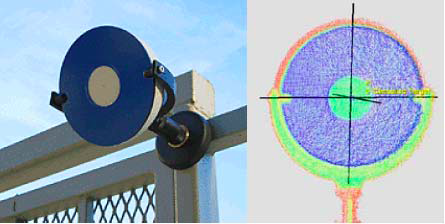
\includegraphics[height=2.5cm]{figure/Chapter7/平面标靶}} \hspace{3em}
			\subfloat{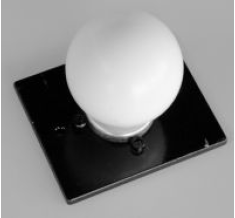
\includegraphics[height=2.5cm]{figure/Chapter7/球形标靶实物}}
			\subfloat{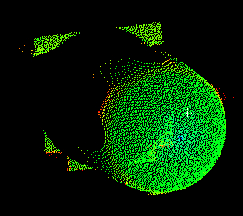
\includegraphics[height=2.5cm]{figure/Chapter7/球形标靶点云}}
			\caption{标靶}
			\label{fig:标靶}
			\hspace{3em}
		\end{figure}
	\item \textbf{三维模型的重建和后处理}
		\begin{itemize}
			\item 利用几何约束或数学上自由曲面函数等方法进行物体曲面的重构;或基于3D TIN方法进行建模;
			\item 由于点云数据有时采集不全或存在噪声,重建后的模型一般还需要进行后处理,如补洞、平滑等。
		\end{itemize}
	\item \textbf{影像与激光点云的配准}有时需要对模型映射真实纹理或者借助影像进行模型的精细重建
		\begin{itemize}
			\item 一般采用数码相机拍摄的真实照片作为纹理来源。
			\item 进行影像与激光点云的配准。
		\end{itemize}
	\item \textbf{纹理映射}
		\begin{itemize}
			\item 前提是实现二维影像与三维模型的配准。
			\item 配准后,将几何模型投影到相应的照片, 即可自动获取纹理坐标, 并进行纹理映射。
			\item 将生成的模型框架输入CAD系统, 人工补充目标的细节。
		\end{itemize}
\end{enumerate}

\section{星载LiDAR系统}

\paragraph{星载激光遥感系统主要应用}
\begin{itemize}
	\item 天体测绘
	\item 全球高程信息的采集
	\item 全球控制点的采集
	\item 环境监测的应用(极地冰盖监测、林业资源调查、大气成分和结构测量)
\end{itemize}

\paragraph{国内外典型星载激光遥感系统}
\begin{itemize}
	\item 用于探测气体溶胶与云层的LITE计划和CALIPSO计划。
	\item 用于天体测绘系统:MOLA-2系统(火星)、Clementine系统(月球)、嫦娥工程(月球)。
	\item 用于极地冰盖监测与大气成分检测的GLAS系统。
\end{itemize}

\paragraph{星载LiDAR数据处理及林业应用}
\begin{itemize}
	\item 星载GLAS波形数据处理:波形参数提取。
	\item 东北地区森林高度反演:基于模拟分析和GLAS波形数据关键参数因子计算,采用回归方程进行森林高度的反演。
	\item 云南森林地上生物量反演:结合机载LiDAR和星载GLAS建立星载GLAS估测森林生物量的模型,利用MERIS反射率数据和全球土地覆盖产品等遥感数据,对LiDAR反演生物量外推,得到的整个研究区的森林地上生物量图。
\end{itemize}